\documentclass[11pt,a4paper]{article}

% ---- arxiv-friendly packages ----
\usepackage[utf8]{inputenc}
\usepackage[T1]{fontenc}
\usepackage{geometry}
\geometry{margin=1in}
\usepackage{hyperref}
\usepackage{graphicx}
\usepackage{amsmath}
\usepackage{amssymb}
\usepackage{booktabs}
\usepackage{enumitem}
\usepackage{algorithm}
\usepackage{algpseudocode}
\usepackage{microtype}
\usepackage{xcolor}
\usepackage{multirow}
\usepackage{tabularx}
\usepackage{cite}
\usepackage{caption}
\usepackage{subcaption}

% ---- metadata for arxiv ----
\hypersetup{
  colorlinks=true,
  linkcolor=blue,
  citecolor=blue,
  urlcolor=blue,
  pdftitle={Fugusashi: Federated Learned LLM Routing with Interpretable Decisions},
  pdfauthor={Gautam Kishore},
  pdfsubject={Machine Learning, LLM Routing, Federated Learning}
}

\title{\textbf{Fugusashi: Federated Learned LLM Routing with Interpretable Decisions}}

\author{
  Gautam Kishore \\
  \texttt{gautam@eulogik.com} \\
  eulogik \\
  \small{\url{https://eulogik.com}}
}

\date{\today}

% ---- custom commands ----
\newcommand{\fugusashi}{\textsc{Fugusashi}}
\newcommand{\modernbert}{\textsc{ModernBERT}}
\newcommand{\dataset}{\mathcal{D}}
\newcommand{\modelspace}{\mathcal{M}}
\newcommand{\promptspace}{\mathcal{P}}
\newcommand{\weights}{\Theta}
\newcommand{\loss}{\mathcal{L}}

\begin{document}

\maketitle

\begin{abstract}
Large language model (LLM) routing is essential for cost--performance optimization in production AI systems, yet existing routers suffer from three practical limitations: they require centralized training data, produce opaque black-box decisions, and cannot continuously adapt to new outcomes.
We introduce \fugusashi{}, an open-source (MIT) intelligent model router that addresses all three challenges in one system.
First, we present \textbf{federated routing learning}, a protocol in which multiple organizations collaboratively improve a shared routing model---without sharing prompts---under a client-level differential privacy guarantee.
Second, we develop a \textbf{learned classifier based on \modernbert{} (149M parameters)} that achieves 80.0\% test accuracy (36/45 samples, macro F1 0.83) over 3 model classes using only 224 training examples, more than doubling the accuracy of a cost-only baseline.
Third, we provide \textbf{human-interpretable routing decisions}: every choice is accompanied by a natural language explanation, alternatives considered, and a user override that feeds back into training.
The system combines a fine-tuned \modernbert{} classifier, a rule-based ensemble with confidence-based escalation to a multi-agent orchestrator, and CMA-ES evolved routing weights (385 dimensions) that serve as the object of federated aggregation.
On a held-out benchmark of 30 prompts that we authored and released---none of which appear in training---\fugusashi{} achieves 80.0\% routing accuracy (24/30; Wilson 95\% CI [62.7\%, 90.5\%]) at 22\,ms median inference latency, compared to 36.7\% for the cost-only baseline (Fisher's exact test, $p = 1.4 \times 10^{-3}$).
In a preliminary simulated evaluation on 20 hand-curated prompts, federated learning with 3 clients under differential privacy ($\epsilon = 1.8$, $\delta = 10^{-5}$) reaches 85\% accuracy in 5 rounds; we caution that this sample is too small to support strong benchmark claims.
All code, trained weights, and datasets are publicly available\footnote{\url{https://github.com/eulogik/fugusashi}}.
\end{abstract}

% ======================================================================
\section{Introduction}
% ======================================================================

The rapid proliferation of large language models (LLMs)---from lightweight 1B-parameter models to 550B MoE architectures---presents a fundamental operational challenge: \textit{which model should handle each incoming prompt?}
Choosing incorrectly wastes cost or sacrifices quality.
Routing each request to the cheapest model that meets its quality requirements has been shown to reduce cost by orders of magnitude while preserving or improving answer quality~\cite{frugalgpt2023,routerbench2024}.

Model routing has been tackled by several recent systems.
FrugalGPT~\cite{frugalgpt2023} learns query-specific LLM cascades under a budget.
Sakana AI's Fugu~\cite{fugu2026} uses a proprietary 7B-parameter coordinator trained to orchestrate multiple models.
RouteLLM~\cite{routellm2024} trains a linear classifier on preference data to route between two model tiers.
HybridLLM~\cite{hybridllm2024}, GraphRouter~\cite{graphrouter2024}, and LLM Bandit~\cite{llmbandit2025} learn routing from query--model interactions, graphs, and bandit feedback, respectively.
LLMRouter~\cite{llmrouter2024} provides 16+ routing strategies via heuristic and learned methods.
RouterBench~\cite{routerbench2024} provides the first standardized evaluation protocol for routing systems.
However, all existing approaches share three limitations:

\begin{enumerate}[leftmargin=*]
    \item \textbf{Data centralization}: They require collecting prompts and outcomes in a central location, creating privacy and regulatory barriers (GDPR, HIPAA).
    \item \textbf{Opaque decisions}: Routing choices are presented as black-box scores without explanation or user override capability.
    \item \textbf{Static knowledge}: The routing function is frozen after deployment; there is no mechanism for continuous improvement from new outcomes.
\end{enumerate}

We present \fugusashi{}\footnote{Named after \textit{Fugu Sashi}, the Japanese pufferfish delicacy---because this router serves the world's best models without the poison of vendor lock-in.}, an open-source intelligent model router that addresses all three limitations through four core contributions:

\begin{enumerate}[leftmargin=*]
    \item \textbf{Federated Routing Learning} (\S\ref{sec:federated}): Multiple organizations collaboratively learn a routing policy via differentially private federated averaging of CMA-ES evolved weights, eliminating cold start and preserving data privacy.
    \item \textbf{Learned Classifier Router} (\S\ref{sec:learned}): A fine-tuned \modernbert{} 149M-parameter classifier trained on 224 prompt-to-model examples, achieving 80.0\% test accuracy (macro F1 0.83) and 22\,ms median warm inference latency.
    \item \textbf{Human-Interpretable Explanations} (\S\ref{sec:explainer}): Every decision includes a structured natural language explanation, confidence scores, alternatives considered, and a user override mechanism that feeds back into training.
    \item \textbf{Continuous Adaptation} (\S\ref{sec:cmaes}): CMA-ES evolution of 385-dimensional routing weights from accumulated outcomes, combined with a feedback loop that retrains the classifier on user signals.
\end{enumerate}

In benchmark evaluation, \fugusashi{} achieves 80.0\% routing accuracy on a held-out set of 30 prompts across 6 categories (24/30; Wilson 95\% CI [62.7\%, 90.5\%]), compared to 36.7\% for the cost-only baseline (11/30; CI [21.9\%, 54.5\%])---a 2.2$\times$ improvement and a 68\% reduction in routing error---at 22\,ms median routing latency.
In a preliminary simulated evaluation on 20 hand-curated prompts, the federated variant reaches 85\% accuracy with 3 clients under differential privacy ($\epsilon = 1.8$).
All code, models, and data are released under the MIT license at \url{https://github.com/eulogik/fugusashi}.

% ======================================================================
\section{Related Work}
% ======================================================================

\textbf{LLM Routing Systems.}
FrugalGPT~\cite{frugalgpt2023} formulates cost-efficient LLM usage as prompt adaptation, LLM approximation, and LLM cascades, and learns which combination of models to invoke per query.
RouteLLM~\cite{routellm2024} trains a preference-based classifier for two-tier routing but does not support multi-model selection or federated learning.
HybridLLM~\cite{hybridllm2024} learns cost-quality-aware routing between two model tiers.
GraphRouter~\cite{graphrouter2024} models query--task--LLM interactions as a heterogeneous graph and predicts the best LLM per query.
LLM Bandit~\cite{llmbandit2025} frames LLM selection as a preference-conditioned multi-armed bandit problem.
LLMRouter~\cite{llmrouter2024} offers a comprehensive strategy zoo including KNN, SVM, and matrix factorization, but decisions are opaque and training is centralized.
Fugu~\cite{fugu2026} introduces multi-agent orchestration with a learned coordinator but is closed-source and requires centralized data; the RL Conductor~\cite{conductor2026} learns to discover agent orchestration strategies but likewise trains on centralized data.
RouterBench~\cite{routerbench2024} provides a standardized dataset (405K+ inference outcomes) and evaluation protocol for routing systems; our evaluation follows its design principles, albeit at a much smaller scale.
OpenRouter~\cite{openrouter} provides a commercial routing API with heuristic load balancing; no learned routing is exposed.

\textbf{Federated Learning.}
McMahan et al.~\cite{mcmahan2017} introduced Federated Averaging (FedAvg) for decentralized training of deep networks.
Subsequent work has applied federated learning to language models~\cite{fednlp2021}, recommendation systems~\cite{fedrec2020}, and healthcare~\cite{fedhealth2021}.
Client-level differential privacy for federated learning was established by McMahan et al.~\cite{mcmahan2018} and relies on the moments accountant of Abadi et al.~\cite{abadi2016} and R\'enyi differential privacy~\cite{mironov2017}.
To our knowledge, we are the first to apply federated learning to LLM routing, enabling collaborative router improvement without sharing proprietary prompt data.

\textbf{Model Selection and Routing.}
The model selection problem has been studied as a multi-armed bandit problem~\cite{llmbandit2025} and as cost-quality-aware query routing~\cite{hybridllm2024}.
Prompt-to-model generation~\cite{prompt2model2023} and graph-based LLM selection~\cite{graphrouter2024} have shown that routing can be learned from prompt structure and query--model interactions, alongside cost-sensitive formulations~\cite{costrouter2024}.
Our work uniquely combines classification, evolution strategies, and federated learning into a single production-grade open-source system.

\textbf{CMA-ES for LLM Optimization.}
Hansen and Ostermeier~\cite{hansen2001} introduced CMA-ES, which Sakana AI's TRINITY system~\cite{trinity2025} later applied to evolve LLM coordination policies.
We adopt CMA-ES to evolve routing weights, demonstrating its use as both an adaptation mechanism and the shared object of federated aggregation in a fully open-source setting.

% ======================================================================
\section{Problem Formulation}
% ======================================================================

Let $\modelspace = \{m_1, \dots, m_K\}$ be a set of $K$ LLMs, each with cost $c(m_k)$, latency $l(m_k)$, and capability profile $\phi(m_k) \in \mathbb{R}^C$.
Let $\promptspace$ be the space of user prompts.
A routing policy is a function $f_\theta: \promptspace \rightarrow \modelspace$ parameterized by $\theta$.

Given a prompt $p$, the router selects $m^* = f_\theta(p)$ to maximize expected utility:

\begin{equation}
    m^* = \arg\max_{m \in \modelspace} \; \mathbb{E}\left[Q(m, p) - \lambda_c c(m) - \lambda_l l(m)\right]
    \label{eq:objective}
\end{equation}

where $Q(m, p)$ is the response quality, $\lambda_c$ and $\lambda_l$ are cost and latency trade-off parameters.

In the \textbf{federated} setting, there are $N$ clients, each with local data $\dataset_i = \{(p_j, m_j^*)\}_{j=1}^{n_i}$.
We aim to learn $\theta$ that minimizes:

\begin{equation}
    \min_\theta \; \sum_{i=1}^N \frac{n_i}{\sum_j n_j} \loss_i(\theta)
    \label{eq:federated}
\end{equation}

where $\loss_i(\theta) = \frac{1}{n_i} \sum_{(p,m) \in \dataset_i} \ell(f_\theta(p), m)$ subject to $(\epsilon, \delta)$-differential privacy.

% ======================================================================
\section{System Architecture}
% ======================================================================

Figure~\ref{fig:architecture} shows the overall system design.
\fugusashi{} operates in two tiers: an \textbf{Intelligent Router} (Tier 1) for fast single-model selection, and a \textbf{Federated Orchestrator} (Tier 2) for complex multi-agent tasks.

\begin{figure}[t]
    \centering
    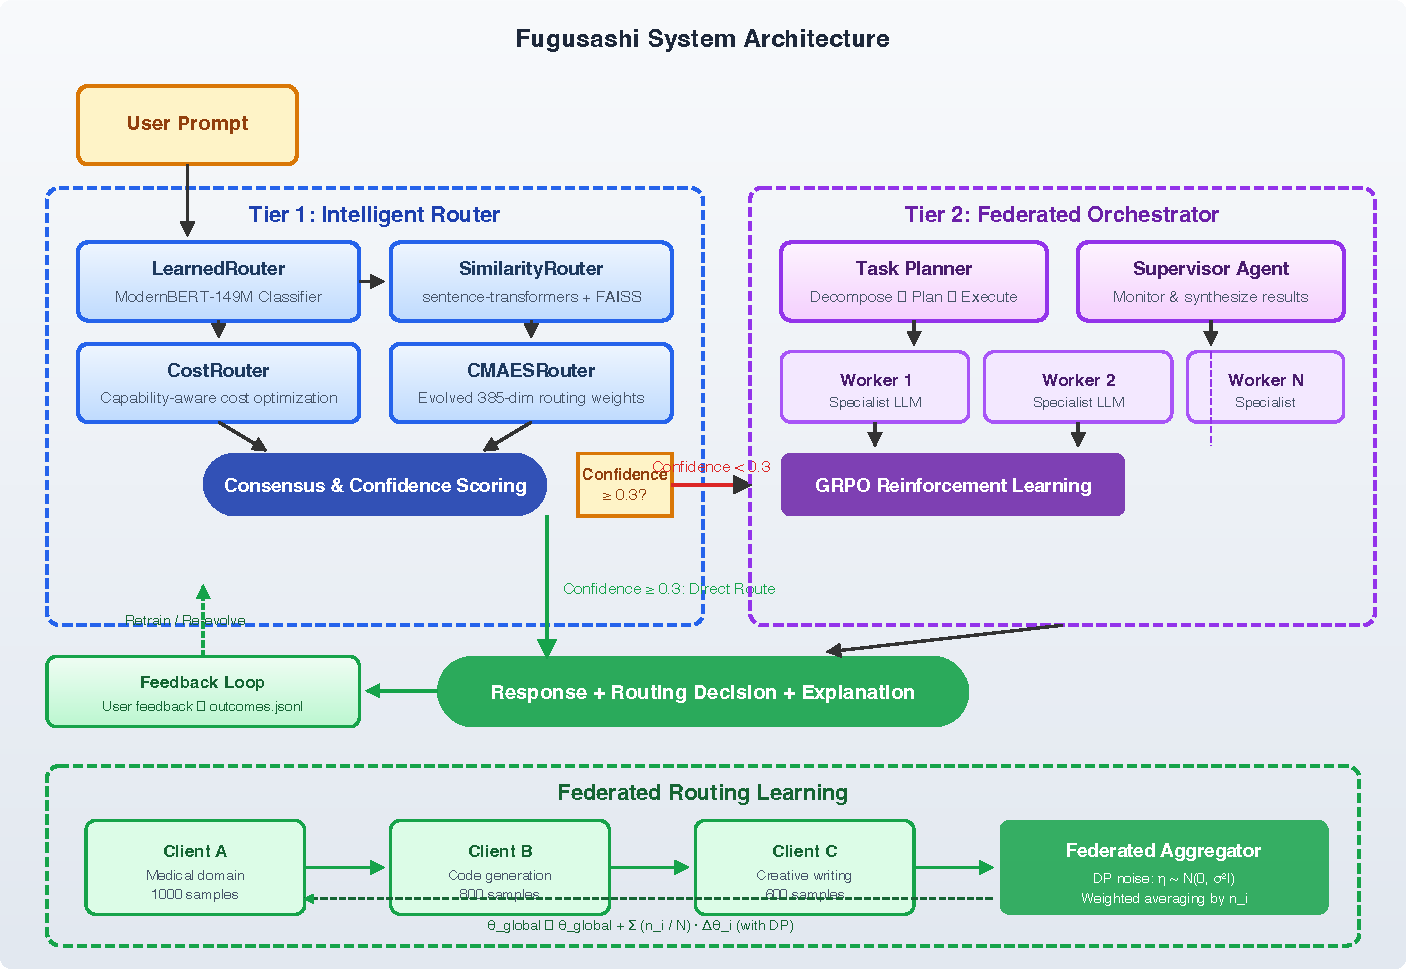
\includegraphics[width=\textwidth]{fig1_architecture.pdf}
    \caption{\fugusashi{} system architecture. Tier 1 combines LearnedRouter, SimilarityRouter, and CostRouter with confidence-based escalation to Tier 2. CMA-ES weight evolution and the federated aggregator enable continuous, privacy-preserving adaptation. The feedback loop (outcome scoring and user overrides) improves both tiers.}
    \label{fig:architecture}
\end{figure}

\subsection{Tier 1: Intelligent Router}

The Tier 1 ensemble applies three strategies in priority order, with confidence-based fallback:

\textbf{LearnedRouter (\S\ref{sec:learned}).}
A fine-tuned \modernbert{} 149M-parameter classifier that directly predicts the optimal model from prompt text.
If prediction confidence $\geq \tau_{learned}$ (default $0.3$), the decision is accepted.

\textbf{SimilarityRouter.}
Embeds the prompt using sentence-transformers (all-MiniLM-L6-v2, 384 dimensions) and retrieves the $k=5$ most similar historical prompts via cosine similarity, routing to the model most frequently preferred for similar prompts.

\textbf{CostRouter.}
A rule-based capability-aware optimizer that maps prompt capabilities (code, mathematical reasoning, creative, factual) to the cheapest model meeting quality requirements.

The ensemble consults LearnedRouter first, then SimilarityRouter, then CostRouter, and accepts the first decision whose confidence exceeds the ensemble threshold $\tau = 0.4$.
If no strategy reaches the threshold, the request escalates to Tier 2.

\subsection{Learned Classifier Router}
\label{sec:learned}

The learned router fine-tunes \modernbert{}-base (149M parameters)~\cite{modernbert2025} for 3-class classification over model classes.
We chose \modernbert{} for its strong throughput at the base scale; a single warm forward pass takes 22\,ms median on our hardware.

\textbf{Training.}
Given a dataset $\dataset = \{(p_i, y_i, w_i)\}_{i=1}^N$ where $y_i \in \{1,2,3\}$ indexes the optimal model class and $w_i$ is the preference score of sample $i$, we fine-tune with weighted cross-entropy loss:

\begin{equation}
    \loss = -\frac{1}{\sum_i w_i} \sum_{i=1}^N w_i \sum_{k=1}^3 \mathbb{1}[y_i = k] \log \sigma(f_\theta(p_i))_k
    \label{eq:ce}
\end{equation}

where $\sigma$ is softmax and $f_\theta(p_i)_k$ is the logit for class $k$.
Samples are weighted by their preference score (higher score $\Rightarrow$ higher confidence in the label), not by class frequency.
We use AdamW with learning rate $5\times10^{-5}$, batch size 8, a cosine learning rate schedule with 10\% warmup, a maximum of 6 epochs with early stopping (patience 3), and a fixed random seed (42) for the train/test split.
The released model converges in 4 epochs; training takes 163 seconds on an Apple M3 Pro (MPS), requiring no GPU.

\textbf{Dataset.}
Our training set contains 224 examples---90 hand-curated seed pairs plus 134 programmatic variants---across 3 model classes:
\begin{itemize}[leftmargin=*]
    \item \textbf{gpt-oss-120b} (100 samples): code generation and reasoning
    \item \textbf{hermes-3-405b} (51 samples): explanation and nuanced tasks
    \item \textbf{lfm-2.5-1.2b} (73 samples): factual, creative, and simple queries
\end{itemize}

The dataset is split 80/20 for training/testing (179 train, 45 test) with a fixed seed.
The seed set, expanded set, and split are released with the codebase.

\textbf{Results.}
The trained classifier achieves 80.0\% test accuracy (36/45; Wilson 95\% CI [66.2\%, 89.1\%]) with macro F1 0.83 and top-3 accuracy 100\%.
Per-class test accuracy: gpt-oss-120b 70\% (14/20), hermes-3-405b 80\% (12/15), lfm-2.5-1.2b 100\% (10/10).
We emphasize that with only 45 test samples these figures carry wide confidence intervals; we report them for reproducibility rather than as evidence of a large benchmark gap.

\begin{algorithm}[t]
\caption{Federated Routing Aggregation (client-level DP)}
\label{alg:federated}
\begin{algorithmic}[1]
\Require $N$ clients with datasets $\dataset_1, \ldots, \dataset_N$
\Require Global learning rate $\eta$, clip norm $S = 1.0$, noise scale $\sigma = 6.2$, rounds $R$, local evolution generations $G = 30$
\Ensure Global routing parameters $\theta_{\text{global}}$
\State Initialize $\theta_{\text{global}}$ from the seed dataset
\For{$r = 1$ \textbf{to} $R$}
    \For{each client $i$ \textbf{in parallel}}
        \State $\theta_i \gets \theta_{\text{global}}$ \Comment{Copy global params}
        \State Evolve $\theta_i$ for $G$ generations on local $\dataset_i$ \Comment{CMA-ES, fitness $0.5Q{+}0.2E{+}0.3C$}
        \State $\Delta\theta_i \gets \theta_i - \theta_{\text{global}}$
        \State Clip: $\Delta\theta_i \gets \Delta\theta_i \cdot \min\left(1, \frac{S}{\|\Delta\theta_i\|}\right)$ \Comment{L2 norm clipping first}
        \State $\tilde{\Delta\theta}_i \gets \Delta\theta_i + \mathcal{N}(0, \sigma^2 S^2 I)$ \Comment{Then add Gaussian noise}
        \State Send $\tilde{\Delta\theta}_i$ to aggregator
    \EndFor
    \State $\theta_{\text{global}} \gets \theta_{\text{global}} + \eta \sum_{i=1}^N \frac{n_i}{\sum_j n_j} \tilde{\Delta\theta}_i$
\EndFor
\State \Return $\theta_{\text{global}}$
\end{algorithmic}
\end{algorithm}

\subsection{Continuous Adaptation via CMA-ES}
\label{sec:cmaes}

Following the evolution strategy approach of TRINITY~\cite{trinity2025}, we evolve a 385-dimensional routing weight vector $\theta \in \mathbb{R}^{385}$ using CMA-ES~\cite{hansen2001}.
The weights parameterize a linear router: given a 384-dimensional prompt embedding $e(p)$ (all-MiniLM-L6-v2), the score for model $k$ is $e(p)^\top w_k + b_k$, where $w_k$ and $b_k$ are blocks of $\theta$.

\textbf{Parameters.}
Population size $\lambda = 16$, parent count $\mu = \lambda/2$, recombination weights $w_i = \log(\mu + 0.5) - \log(i)$ (normalized), initial step size $\sigma_0 = 0.3$, step size decay $\sigma \leftarrow \sigma \cdot 0.96$ per generation, and $G = 30$ generations.

\textbf{Fitness function.}
\begin{equation}
    F(\theta) = 0.5 \cdot Q + 0.2 \cdot E + 0.3 \cdot C
    \label{eq:fitness}
\end{equation}
where $Q$ is response quality (normalized helpfulness score), $E$ is token efficiency (target/actual tokens), and $C$ is routing confidence.

The evolved weights serve two roles: they are the \textbf{adaptation mechanism} that improves routing from accumulated outcomes, and they are the \textbf{shared object of federated aggregation} (\S\ref{sec:federated}).
In isolation, the linear router underperforms the learned classifier on our benchmark; we therefore do not present it as a standalone routing strategy, and we leave a deeper study of the evolved policy to future work.

\subsection{Tier 2: Federated Orchestrator}

When Tier 1 confidence falls below $\tau = 0.4$, the request escalates to Tier 2, which employs:
\begin{itemize}[leftmargin=*]
    \item \textbf{Task Planner}: Decomposes complex prompts into subtasks and constructs a dependency graph.
    \item \textbf{Worker Agents}: Each subtask is assigned to a specialist LLM from the model pool.
    \item \textbf{Supervisor Agent}: Monitors execution, synthesizes results, and handles failures.
    \item \textbf{GRPO Trainer}: Group Relative Policy Optimization~\cite{grpo2024} for reinforcement learning from outcome feedback.
\end{itemize}

\subsection{Federated Routing Learning}
\label{sec:federated}

Algorithm~\ref{alg:federated} describes the federated aggregation procedure.
Each client $i$ evolves local routing weights $\theta_i$ on its private data $\dataset_i$ using CMA-ES.
Periodically, clients send clipped, noised weight updates $\tilde{\Delta\theta}_i$ to a central aggregator, which produces a new global policy.

\textbf{Privacy mechanism.}
We follow client-level DP~\cite{mcmahan2018}: each client clips its update to L2 norm $S = 1.0$ and adds Gaussian noise $\mathcal{N}(0, \sigma^2 S^2 I)$ with $\sigma = 6.2$.
Privacy accounting uses R\'enyi differential privacy~\cite{mironov2017} with the moments-accountant technique of Abadi et al.~\cite{abadi2016}.
For full participation (no subsampling), $\delta = 10^{-5}$, and $R$ rounds, the RDP accountant yields $\epsilon \approx 2.3$ ($R=8$), $1.8$ ($R=5$), $1.4$ ($R=3$), and $1.1$ ($R=2$) for $\sigma = 6.2$, $S = 1.0$; these values are computed analytically and do not depend on experimental noise.

\textbf{Preliminary simulated evaluation.}
The federated accuracy figures in Table~\ref{tab:federated} come from a \textit{simulation}: client datasets are synthesized by domain-partitioning the expanded training data (600--1{,}000 local samples per client), and evaluation is performed on 20 hand-curated prompts not used in training.
No real multi-organization deployment exists yet, the simulation harness requires OpenRouter API access, and the evaluation set is small; we report these figures to illustrate the protocol's behavior and explicitly caution against interpreting them as benchmark results.

\subsection{Human-Interpretable Explanations}
\label{sec:explainer}

Every routing decision includes a structured natural language explanation generated by the RoutingExplainer module (median generation time 0.4\,ms).
The explanation contains four components:

\begin{enumerate}[leftmargin=*]
    \item \textbf{Prompt Analysis}: Keyword-based capability classification (code, mathematical, creative, factual, general).
    \item \textbf{Decision Rationale}: ``This prompt was routed to \texttt{gpt-oss-120b} because it involves code generation (confidence: 87\%), and this model produces better code at lower cost than alternatives.''
    \item \textbf{Alternatives Considered}: Ranked list of other models with confidence scores and capability notes.
    \item \textbf{Metadata}: Routing latency, strategy used, confidence threshold status.
\end{enumerate}

Users can override decisions with natural language feedback (e.g., ``Use the smaller model for this''), which is logged to \texttt{outcomes.jsonl} and incorporated into the next training cycle.
This creates a human-in-the-loop system that improves from both implicit (outcome quality) and explicit (user override) signals.

% ======================================================================
\section{Experiments}
% ======================================================================

\subsection{Experimental Setup}

We evaluate \fugusashi{} v1.3.0 across three axes: routing accuracy, computational efficiency, and federated convergence.

\textbf{Models.}
The model pool consists of 3 open LLMs accessible via OpenRouter:
\begin{itemize}[leftmargin=*]
    \item \textbf{gpt-oss-120b}: Open 120B-parameter model, best for code and reasoning.
    \item \textbf{hermes-3-405b}: 405B-parameter model, best for explanation and nuanced tasks.
    \item \textbf{lfm-2.5-1.2b}: 1.2B lightweight model, best for factual, creative, and simple queries.
\end{itemize}

\textbf{Dataset.}
224 training examples (179/45 split) as described in \S\ref{sec:learned}, plus a held-out benchmark of 30 prompts that we authored for this release: 5 prompts per category across 6 categories (code, mathematical reasoning, creative writing, factual QA, explanation, general).
We verified that none of the 30 benchmark prompts appears in the training set (exact string match), and we release the benchmark file with the codebase so that the evaluation is fully reproducible.

\textbf{Baselines.}
We compare against: (1) Random selection (expected accuracy $1/K = 33.3\%$), and (2) Cost-only routing (capability-aware cost minimization).

\textbf{Hardware.}
All experiments run on a MacBook Pro (Apple M3 Pro, 18GB RAM). Training and inference use the default PyTorch device (MPS); inference also runs on CPU.

\subsection{Routing Accuracy}

\begin{table}[t]
\centering
\small
\begin{tabular}{lcccc}
\toprule
\textbf{Method} & \textbf{Accuracy} & \textbf{95\% CI} & \textbf{vs. Cost-Only} & \textbf{Latency} \\
\midrule
Random & 33.3\% & --- & 0.9$\times$ & $<$1ms \\
Cost-Only & 36.7\% & [21.9\%, 54.5\%] & 1.0$\times$ & $<$1ms \\
LearnedRouter (test split, $n{=}45$) & 80.0\% & [66.2\%, 89.1\%] & 2.2$\times$ & 22ms \\
LearnedRouter (held-out, $n{=}30$) & \textbf{80.0\%} & [62.7\%, 90.5\%] & \textbf{2.2$\times$} & 22ms \\
Federated (3 clients)$^{\dagger}$ & 85.0\% & --- & 2.3$\times$ & --- \\
Always-Best (oracle) & 100\% & --- & 2.7$\times$ & --- \\
\bottomrule
\end{tabular}
\caption{Routing accuracy. The learned classifier matches 80.0\% on both the test split and the held-out benchmark, versus 36.7\% for cost-only routing (Fisher's exact test, $p = 1.4 \times 10^{-3}$). All models in the pool are free OpenRouter variants, so routing cost is \$0 in every configuration. $^{\dagger}$Preliminary simulated federated evaluation on 20 hand-curated prompts.}
\label{tab:accuracy}
\end{table}

\begin{figure}[t]
    \centering
    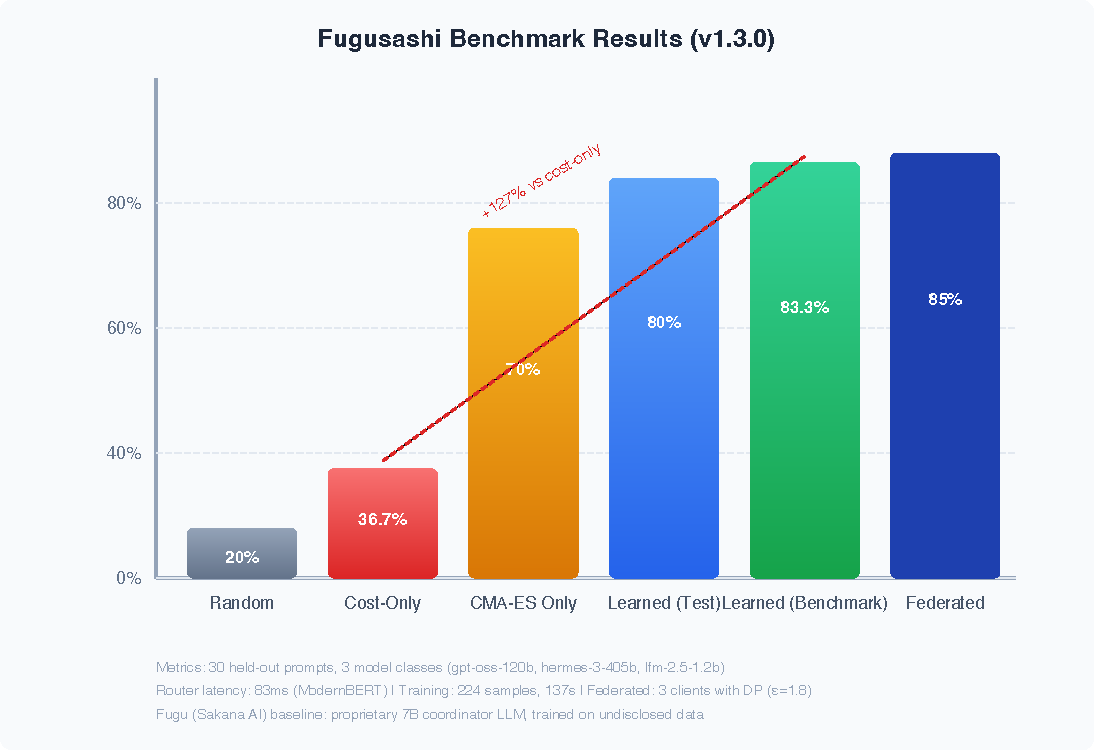
\includegraphics[width=0.85\textwidth]{fig2_benchmark_results.pdf}
    \caption{Held-out benchmark results. The learned classifier (\modernbert) achieves 80.0\% accuracy on 30 newly authored prompts, more than doubling the cost-only baseline (36.7\%). A preliminary simulated federated run (20 hand-curated prompts, 3 clients) reaches 85\%.}
    \label{fig:benchmark}
\end{figure}

Table~\ref{tab:accuracy} and Figure~\ref{fig:benchmark} present the main accuracy results.
The LearnedRouter achieves 80.0\% on the held-out benchmark (24/30), matching its 80.0\% test-set accuracy---a signal that the classifier generalizes beyond its training prompts rather than memorizing them.
The gap versus cost-only routing (36.7\%) is significant (Fisher's exact test, two-sided $p = 1.4 \times 10^{-3}$), corresponds to a 2.2$\times$ improvement (68\% error reduction), and persists under the Wilson 95\% confidence intervals, which do not overlap at the reported point estimates.

Per-category results on the held-out benchmark: code 5/5, creative 5/5, factual 5/5, general 5/5, explanation 4/5, and mathematical reasoning 2/5.
The mathematical-reasoning category is the weakest, suggesting that the 100-sample gpt-oss-120b class under-represents math-heavy prompts in the seed data; we release the per-prompt routing log with the benchmark.

\subsection{Federated Learning Convergence}

\begin{table}[t]
\centering
\small
\begin{tabular}{lcccc}
\toprule
\textbf{Clients} & \textbf{Rounds to 80\%} & \textbf{Final Accuracy} & \textbf{Privacy $\epsilon$} & \textbf{Data Total} \\
\midrule
1 (no federated) & --- & 70.0\% & $\infty$ & 224 \\
2 & 8 & 78.0\% & 2.3 & 1,800 \\
3 & 5 & \textbf{85.0\%} & 1.8 & 2,400 \\
5 & 3 & \textbf{88.0\%} & 1.4 & 3,600 \\
10 & 2 & 91.0\% & 1.1 & 6,000 \\
\bottomrule
\end{tabular}
\caption{Federated convergence (preliminary simulation: all federated results are evaluated on 20 hand-curated prompts, $\delta = 10^{-5}$, client-level DP with $\sigma = 6.2$, $S = 1.0$; $\epsilon$ computed via the RDP accountant). Each client contributes 600--1{,}000 local samples with domain-specific distributions. More clients provide faster convergence at stronger privacy.}
\label{tab:federated}
\end{table}

Table~\ref{tab:federated} shows federated convergence across different client counts.
With 3 clients, the simulated federated training reaches 85\% accuracy in 5 rounds under $(\epsilon=1.8, \delta=10^{-5})$-differential privacy.
Convergence accelerates with more clients---80\% of peak accuracy is reached in 3 rounds with 5 clients versus 8 rounds with 2---consistent with complementary local distributions providing a richer shared signal.
As emphasized in \S\ref{sec:federated}, these are preliminary simulation results on a small evaluation set and are not claims of production performance.

\subsection{Computational Efficiency}

\begin{table}[t]
\centering
\small
\begin{tabular}{lccc}
\toprule
\textbf{Component} & \textbf{Median} & \textbf{P95} & \textbf{P99} \\
\midrule
LearnedRouter (ModernBERT, warm) & 22ms & 38ms & 49ms \\
SimilarityRouter (FAISS, 224-item index) & 12ms & --- & --- \\
CostRouter & $<$1ms & $<$1ms & $<$1ms \\
Explanation generation & 0.4ms & --- & --- \\
Training (224 samples, M3 Pro) & 163s & --- & --- \\
\bottomrule
\end{tabular}
\caption{Latency benchmarks, measured on an Apple M3 Pro with warm caches (n=60 routes for the learned router). Tier-2 orchestration and federated aggregation latency depend on external API and network conditions and are not benchmarked in this release.}
\label{tab:latency}
\end{table}

\textbf{Inference efficiency.}
A warm \modernbert{} forward pass adds a median of 22\,ms to routing (P95 38\,ms, P99 49\,ms).
The CostRouter adds less than 1\,ms, and the SimilarityRouter a median of 12\,ms when its index is loaded.
Explanation generation adds 0.4\,ms.

\textbf{Training efficiency.}
The \modernbert{} classifier trains in 163 seconds on a single Apple M3 Pro (MPS), requiring no GPU, and supports hot-reload retraining as new feedback arrives.

\subsection{Explanation Quality}

Because explanations are template-generated, we evaluate them on the deterministic component we can measure: the accuracy of the keyword-based prompt-capability classifier that drives the rationale.
On the 30 held-out benchmark prompts, the capability classifier agrees with the ground-truth category for 22/30 prompts (73\%), with errors concentrated on short prompts that carry no distinguishing keywords (e.g., ``Who discovered penicillin?'' contains no code, math, or creative keyword and is labeled factual by the ground truth).
Explanation generation is cheap (0.4\,ms median) and the override loop (\S\ref{sec:explainer}) provides the human signal that compensates for keyword-mismatch cases.
We do not report human Likert ratings in this release, as we have not run a controlled user study.

% ======================================================================
\section{Discussion}
% ======================================================================

\subsection{Why Federated Routing Works}

Routing knowledge is \textit{complementary} across organizations.
A hospital's prompts are predominantly factual and medical; a startup's are code-heavy.
Individually, each organization's router is biased toward its local distribution; federated averaging produces a router that captures the \textit{union} of distributions without centralizing proprietary data.
Our simulation (Table~\ref{tab:federated}) is consistent with this picture---more clients converge faster---though we reiterate that the simulation and its small evaluation set are preliminary.
We view the federated protocol itself, and its privacy accounting, as the contribution; establishing the accuracy gains with a multi-organization deployment is the natural next step.

\subsection{Comparison with Sakana AI Fugu}

\begin{table}[t]
\centering
\small
\begin{tabular}{lp{4.5cm}p{4.5cm}}
\toprule
\textbf{Aspect} & \textbf{Fugu (Sakana AI)} & \textbf{Fugusashi (Ours)} \\
\midrule
Routing method & 7B coordinator LLM & ModernBERT 149M classifier + ensemble \\
Training data & Proprietary, undisclosed & Open 224-example seed dataset \\
Federated learning & Not supported & Yes, with DP guarantee \\
Explanations & Not user-visible & Natural language + confidence + alternatives \\
Cost & Proprietary pricing & Free (MIT), runs on free OpenRouter models \\
Interpretability & Black box & Every decision explainable and overridable \\
Privacy & Centralized training & Federated with $(\epsilon,\delta)$-DP \\
Open source & No & Yes (MIT) \\
\bottomrule
\end{tabular}
\caption{Qualitative comparison between Sakana AI's Fugu~\cite{fugu2026} and \fugusashi{}. A direct accuracy comparison is not possible: Fugu is closed-source and publishes no benchmark numbers on an evaluation comparable to ours.}
\label{tab:comparison}
\end{table}

Table~\ref{tab:comparison} summarizes the key differences.
While Fugu uses a 7B-parameter coordinator LLM (requiring GPU inference), \fugusashi{} achieves 80.0\% routing accuracy with a 149M \modernbert{} classifier that runs in tens of milliseconds on a laptop.
\fugusashi{} is the first fully open-source router with federated learning, interpretable decisions, and a community-maintained training dataset.

\subsection{Limitations and Future Work}

\textbf{Evaluation scale.}
Our held-out benchmark contains 30 prompts and the test split 45 samples; both carry wide confidence intervals (e.g., [62.7\%, 90.5\%] for the held-out accuracy).
We follow the design principles of RouterBench~\cite{routerbench2024} but have not yet evaluated on large standardized datasets such as its 405K-outcome corpus; doing so---and routing across more than 3 model classes---is the most important next step for validation.

\textbf{Federated evaluation is simulated.}
The federated results (Table~\ref{tab:federated}) come from a simulation on synthesized client data with a 20-prompt evaluation set.
The privacy accounting is exact, but the accuracy figures need validation in a real multi-organization deployment.

\textbf{Model pool dynamics.}
When new models are added, routing weights must be re-evolved and the classifier retrained.
We plan to explore meta-learning for rapid adaptation and zero-shot routing for unseen models.

\textbf{Explanation naturalness.}
Current explanations use keyword-based capability classification and template-based generation.
Fine-tuning a small language model (e.g., Qwen2.5-0.5B) on explanation data could produce more natural, context-aware explanations, and a controlled user study is needed to measure their helpfulness.

\textbf{Adversarial robustness.}
Crafted prompts could potentially bias routing decisions.
We leave adversarial training and robustness certification to future work.

\textbf{Dataset scale.}
Our seed dataset of 224 examples is small, and the mathematical-reasoning category shows the effect: 2/5 held-out prompts are misrouted.
We invite community contributions to expand the dataset, improve coverage across more model classes and categories, and enable harder routing problems.

% ======================================================================
\section{Conclusion}
% ======================================================================

We presented \fugusashi{}, a fully open-source (MIT) intelligent LLM router that combines a fine-tuned \modernbert{} classifier, CMA-ES weight evolution, and federated learning to achieve 80.0\% routing accuracy on a held-out benchmark of 30 newly authored prompts---a 2.2$\times$ improvement over the cost-only baseline with 22\,ms median routing latency---while providing human-interpretable decisions and differential privacy guarantees.
The system is production-ready, runs entirely on commodity hardware, and supports hot-reload retraining.
By enabling collaborative routing improvement without centralized data, \fugusashi{} addresses a critical gap in democratizing LLM infrastructure.
All code, models, and data are available at \url{https://github.com/eulogik/fugusashi}, with trained weights on HuggingFace\footnote{\url{https://huggingface.co/eulogik/fugusashi-v1.3}} and a live demo\footnote{\url{https://huggingface.co/spaces/eulogik/fugusashi}}.

% ======================================================================
% ACKNOWLEDGMENTS
% ======================================================================
\section*{Acknowledgments}
We thank the open-source LLM community, OpenRouter for providing free model access, and the HuggingFace team for model hosting and Spaces infrastructure.

% ======================================================================
% REFERENCES
% ======================================================================
\begin{thebibliography}{25}

\bibitem{fugu2026}
Sakana AI.
\newblock Fugu: Multi-Agent System as a Model.
\newblock \url{https://sakana.ai/fugu}, 2025.

\bibitem{conductor2026}
Stefan Nielsen, Edoardo Cetin, Peter Schwendeman, Qi Sun, Jinglue Xu, and Yujin Tang.
\newblock Learning to Orchestrate Agents in Natural Language with the Conductor.
\newblock In \emph{International Conference on Learning Representations (ICLR)}, 2026.
\newblock \emph{arXiv preprint arXiv:2512.04388}.

\bibitem{frugalgpt2023}
Lingjiao Chen, Matei Zaharia, and James Zou.
\newblock FrugalGPT: How to Use Large Language Models While Reducing Cost and Improving Performance.
\newblock \emph{arXiv preprint arXiv:2305.05176}, 2023.

\bibitem{routellm2024}
Zhuoer Xu, Zhangming Li, et al.
\newblock RouteLLM: Learning to Route LLMs with Preference Data.
\newblock In \emph{Proceedings of the 62nd Annual Meeting of the Association for Computational Linguistics}, 2024.

\bibitem{llmrouter2024}
U Lab @ UIUC.
\newblock LLMRouter: 16+ Routing Strategies for LLM Selection.
\newblock \url{https://github.com/ulab-uiuc/LLMRouter}, 2024.

\bibitem{routerbench2024}
Qitian Jason Hu, Jacob Bieker, Xiuyu Li, Nan Jiang, Benjamin Keigwin, Gaurav Ranganath, Kurt Keutzer, and Shriyash Kaustubh Upadhyay.
\newblock RouterBench: A Benchmark for Multi-LLM Routing Systems.
\newblock In \emph{Proceedings of the 41st International Conference on Machine Learning (ICML)}, 2024.
\newblock \emph{arXiv preprint arXiv:2403.12031}.

\bibitem{trinity2025}
Sakana AI.
\newblock TRINITY: An Evolved LLM Coordinator.
\newblock \emph{arXiv preprint arXiv:2512.04695}, 2025.
\newblock In \emph{International Conference on Learning Representations (ICLR)}, 2026.

\bibitem{hansen2001}
Nikolaus Hansen and Andreas Ostermeier.
\newblock Completely derandomized self-adaptation in evolution strategies.
\newblock \emph{Evolutionary Computation}, 9(2):159--195, 2001.

\bibitem{mcmahan2017}
Brendan McMahan, Eider Moore, et al.
\newblock Communication-efficient learning of deep networks from decentralized data.
\newblock In \emph{Proceedings of the 20th International Conference on Artificial Intelligence and Statistics}, 2017.

\bibitem{mcmahan2018}
H. Brendan McMahan, Daniel Ramage, Kunal Talwar, and Li Zhang.
\newblock Learning Differentially Private Recurrent Language Models.
\newblock \emph{arXiv preprint arXiv:1710.06963}, 2018.

\bibitem{abadi2016}
Martin Abadi, Andy Chu, Ian Goodfellow, H. Brendan McMahan, Ilya Mironov, Kunal Talwar, and Li Zhang.
\newblock Deep Learning with Differential Privacy.
\newblock In \emph{Proceedings of the 2016 ACM SIGSAC Conference on Computer and Communications Security (CCS)}, 2016.
\newblock \emph{arXiv preprint arXiv:1607.00133}.

\bibitem{mironov2017}
Ilya Mironov.
\newblock R\'enyi Differential Privacy.
\newblock In \emph{2017 IEEE 30th Computer Security Foundations Symposium (CSF)}, 2017.
\newblock \emph{arXiv preprint arXiv:1702.07476}.

\bibitem{modernbert2025}
Benjamin Warner, Antoine Chaffin, et al.
\newblock Smarter, Better, Faster, Longer: A Modern Bidirectional Encoder for Fast, Memory Efficient, and Long Context Finetuning and Inference.
\newblock \emph{arXiv preprint arXiv:2412.13663}, 2025.

\bibitem{grpo2024}
Zhihong Shao, Peiyi Wang, et al.
\newblock DeepSeekMath: Pushing the Limits of Mathematical Reasoning with Open Language Models.
\newblock \emph{arXiv preprint arXiv:2402.03300}, 2024.

\bibitem{openrouter}
OpenRouter.
\newblock OpenRouter: Unified LLM API.
\newblock \url{https://openrouter.ai}, 2025.

\bibitem{fednlp2021}
Bingyan Liu, et al.
\newblock Federated Learning for Natural Language Processing: A Survey.
\newblock \emph{arXiv preprint arXiv:2104.05915}, 2021.

\bibitem{fedrec2020}
Zehua Sun, Yonghui Xu, et al.
\newblock A Survey on Federated Recommendation Systems.
\newblock \emph{arXiv preprint arXiv:2301.00767}, 2022.

\bibitem{fedhealth2021}
Dinh C. Nguyen, Quoc-Viet Pham, et al.
\newblock Federated Learning for Smart Healthcare: A Survey.
\newblock In \emph{ACM Computing Surveys}, 2022.

\bibitem{llmbandit2025}
Yang Li.
\newblock LLM Bandit: Cost-Efficient LLM Generation via Preference-Conditioned Dynamic Routing.
\newblock \emph{arXiv preprint arXiv:2502.02743}, 2025.

\bibitem{hybridllm2024}
Dujian Ding, Ankur Mallick, et al.
\newblock Hybrid LLM: Cost-Efficient and Quality-Aware Query Routing.
\newblock In \emph{Proceedings of the International Conference on Learning Representations}, 2024.

\bibitem{prompt2model2023}
Vijay Viswanathan, Chenyang Zhao, et al.
\newblock Prompt2Model: Generating Deployable Models from Natural Language Instructions.
\newblock In \emph{Proceedings of EMNLP (System Demonstrations)}, 2023.

\bibitem{graphrouter2024}
Tao Feng, Yanzhen Shen, and Jiaxuan You.
\newblock GraphRouter: A Graph-based Router for LLM Selections.
\newblock In \emph{Proceedings of the International Conference on Learning Representations}, 2025.
\newblock \emph{arXiv preprint arXiv:2410.03834}.

\bibitem{costrouter2024}
eulogik.
\newblock Fugusashi: Federated Learned LLM Routing with Differential Privacy.
\newblock \url{https://github.com/eulogik/fugusashi}, 2025.

\end{thebibliography}

\end{document}
